\section*{Supplementary materials}

\begin{figure}[ht]
    \centering
    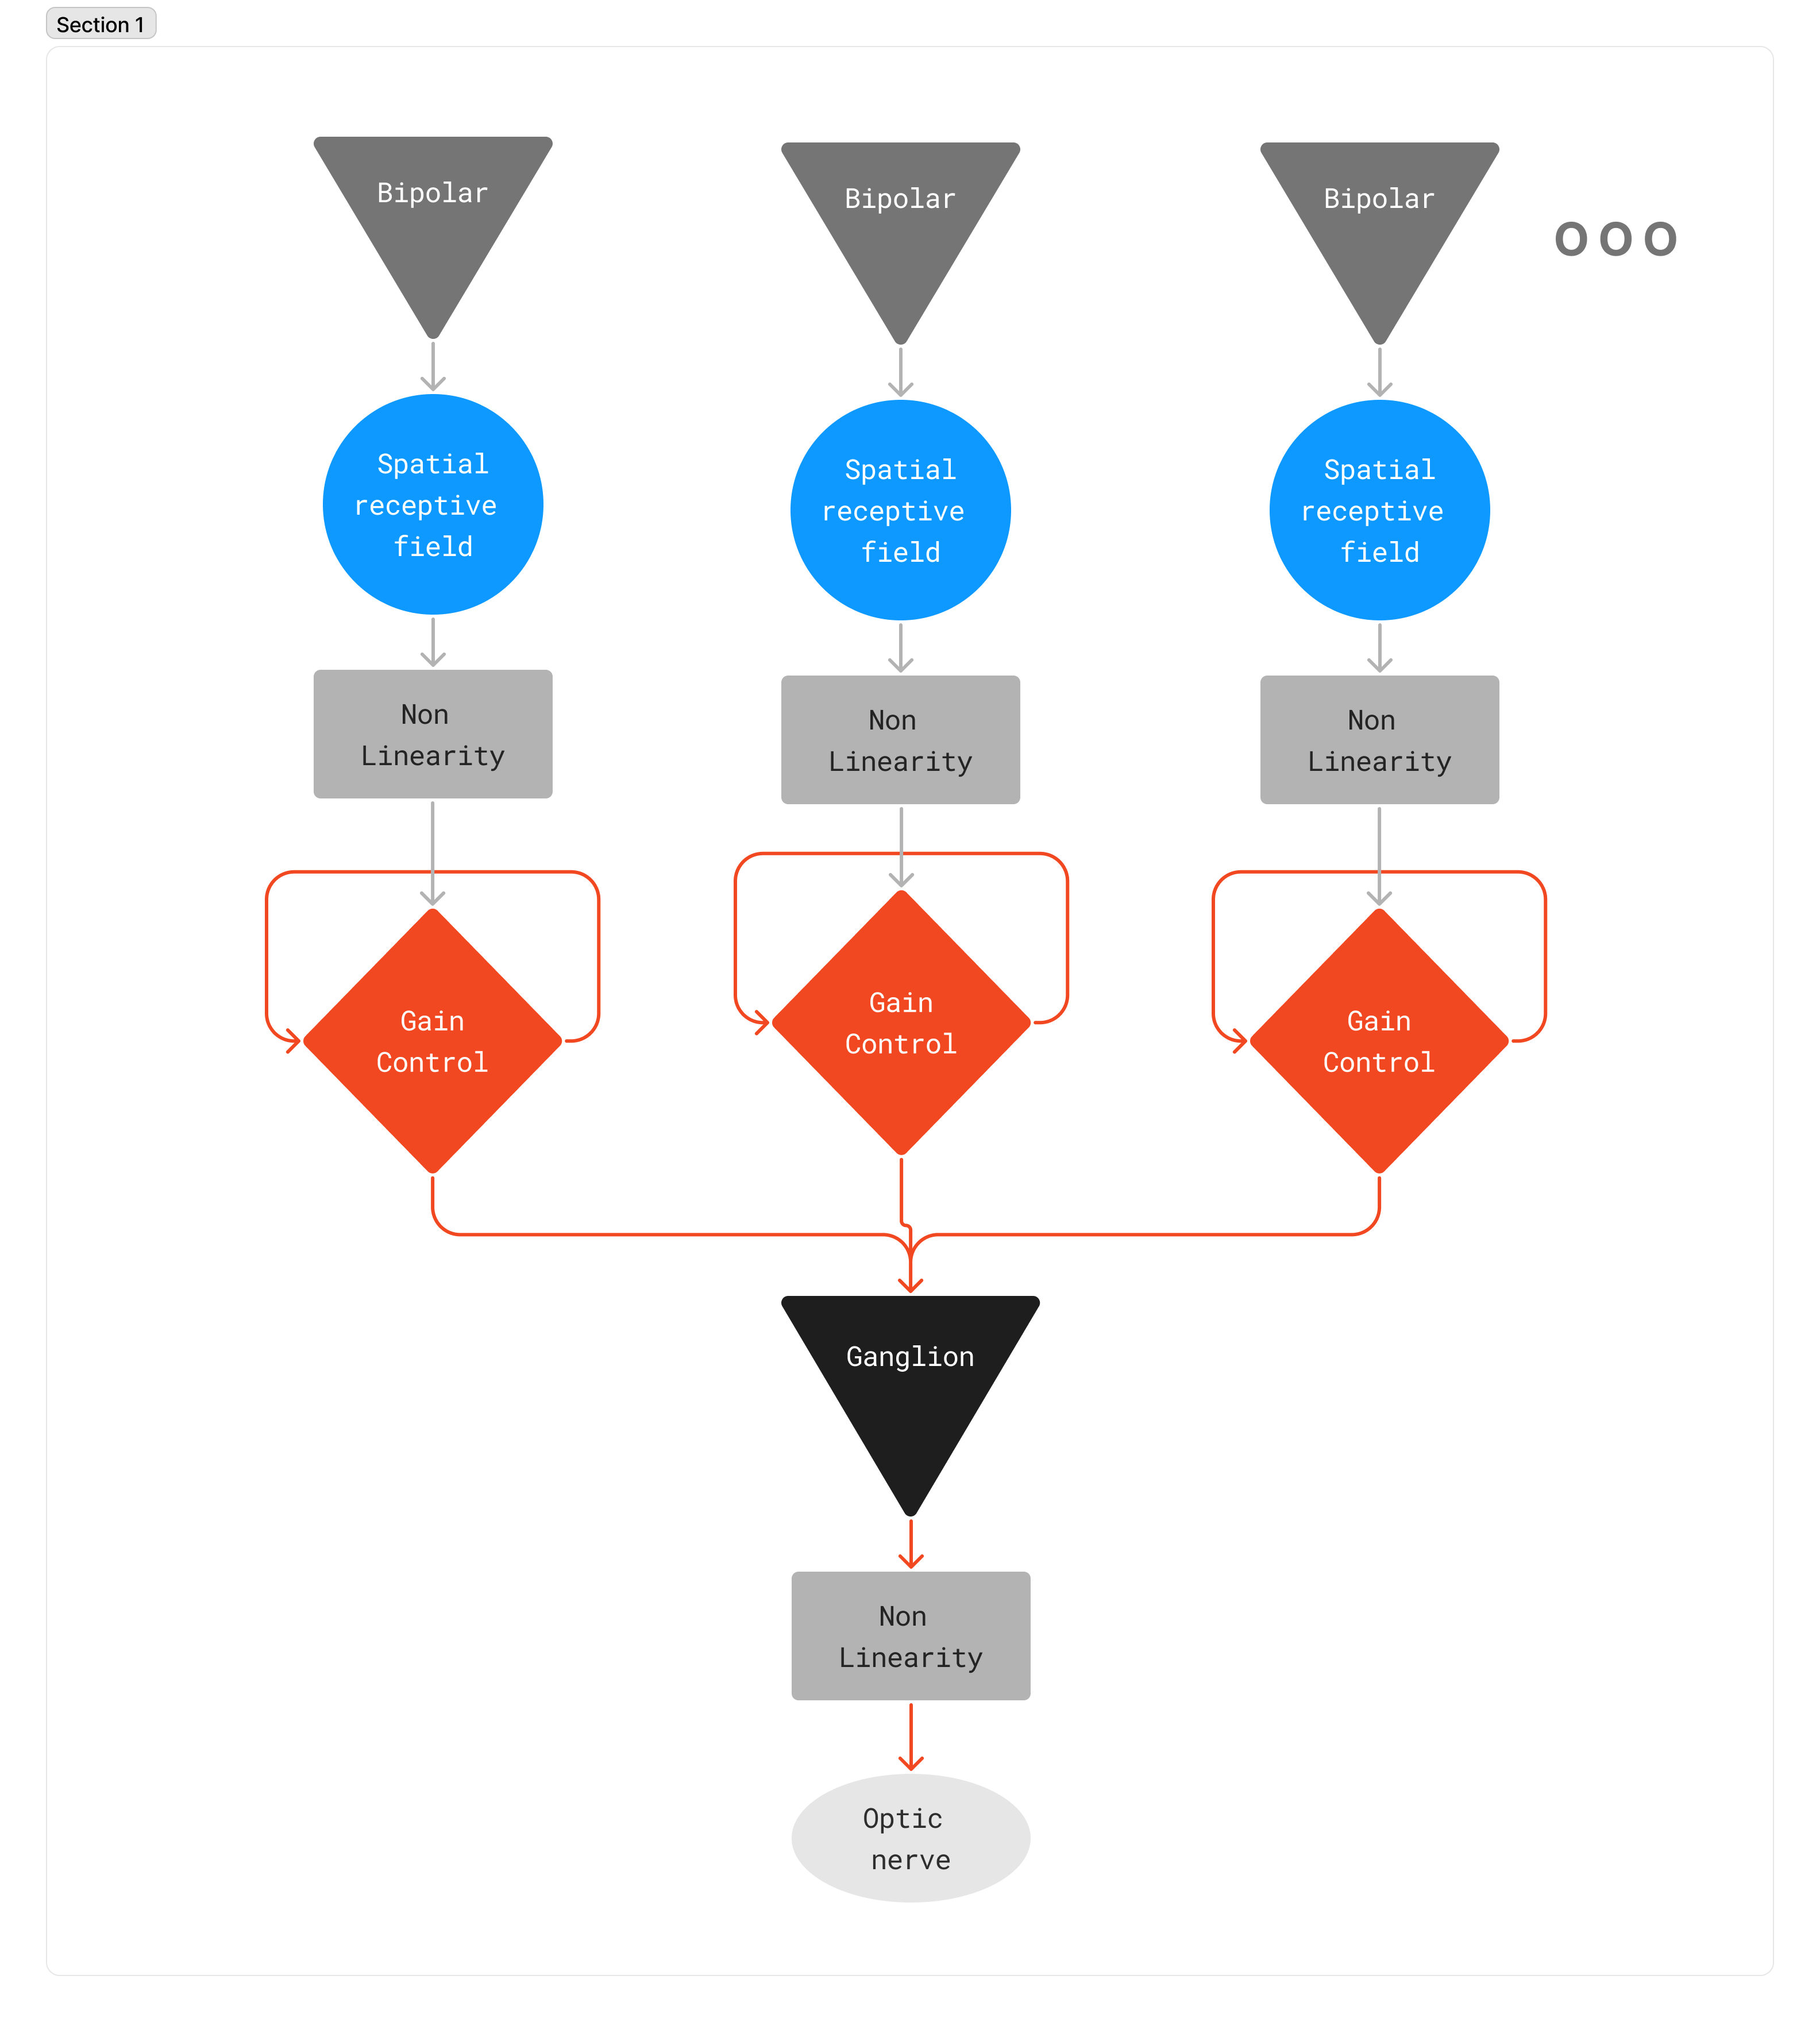
\includegraphics[width=\textwidth]{pics/GCModelDiagram.png}
    \caption{\textbf{Quick sketch of a gain control LNLN model.} Each bipolar
        cell is
        composed of a linear spatial filter that selectively responds to part
        of the scene,
        a non-linear activation function, and a gain control mechanism that
        scale its output
        depending on past events. They all converge into on bipolar cell
        (forming its receptive field)
        of which output is also modeled using a non-linear function.}
    \label{fig:LNLN}
\end{figure}